\documentclass[titlepage]{article}
\usepackage[utf8]{inputenc}
\usepackage{graphicx,verbatim,amsmath,amssymb,amsthm}
\usepackage{subcaption}
\usepackage{titlepic}

\title{Implementing Deep Q Learning and Double Deep Q learning in training Pac-Man \\
\titlepic{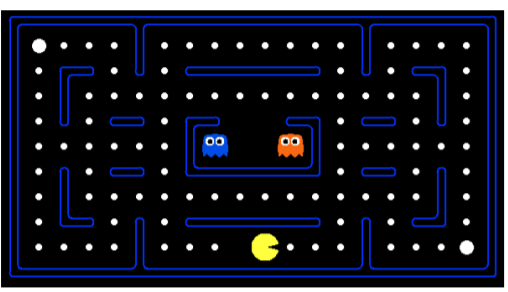
\includegraphics[width=\textwidth]{images/pacman.png}}
\ \\
\large {Final Project: Project Proposal}\\
\ \\
ECE 517 - Reinforcement Learning \\
Prof. Dr. Amir Sadovnik
}

\author{Jerry Duncan, Fabian Fallas, Tabitha Samuel }
\date{November 2020}


\begin{document}

\maketitle
\section{Problem definition}
Using reinforcement learning techniques to teach algorithms to `play' Atari games has been a popular and constantly evolving research area in the past five years. For this final project, we propose to use Deep Q-Learning, and double deep Q-Learning reinforcement learning techniques to train a model to successfully play the Pac-Man game. We will follow Gnanasekaran et al. \cite{gnanasekaranreinforcement} in condensing the Pac-Man grid into a $n \times m$ image where each pixel represents a possible state (e.g. one color will represent walls, another the ghosts, etc). We will initially train the models on the small grid provided by \cite{pacman}, and then compare change in complexity and run-time when they are run on the medium sized grid.

\section{Problem motivation and background}
Most research problems are usually supervised tasks that need the regular pipelines of training and testing. Also, traditionally these tasks are applied over environments that are ``static'', that is, the data helps to tune the weights and the resulting model can be applied over the validation set. But with reinforcement learning we can apply algorithms to dynamic and evolving environments and, as in the case of video games, the artificial intelligence can be seen in action - in a way that is not just responding to a static environment. Consequently, we want to use video games in order to experience how an agent can play the game without human intervention. By doing this project we will face the following challenges:
\begin{itemize}
  \item Program our first function approximation algorithms.
  \item Use an interface for video games.
  \item Use Deep Q-Learning which is a well-noted solution for complex tasks.
  \item Understand and program Double Deep Q-Learning.
\end{itemize}

We propose to build upon the work described in \cite{gnanasekaranreinforcement}. In this paper, the group investigates the effectiveness of Deep Q-learning based on the context of the Pac-Man game using Q-learning and Approximate Q-learning as baselines. We plan on implementing Deep Q learning, and adding an additional model with Double Deep Q learning, and comparing performance and accuracy trade offs between the two techniques. We also plan on adding prioritized experience replay to see if we can increase the speed in which our models learn, using both \cite{schaul2016prioritized} and some of our own intuitions of which experience to replay.

\section{Evaluation of results}
We would like to evaluate results from three perspectives in this project:
\begin{itemize}
  \item Evaluate increase in complexity and training time when we move from the small grid to the medium sized grid.
  \item Compare performance of Deep Q-learning versus Double Deep Q-learning. By using Double Q-Learning we will implement something different from \cite{gnanasekaranreinforcement}.
  \item Attempt to add prioritized replay in the way described by \cite{schaul2016prioritized} and separately using some of our own ideas.
\end{itemize}

If time permits we would like to create an implementation of regular Q-Learning. This can be interesting since by using this implementation uses a simpler function approximation.

\bibliographystyle{IEEEtran}
\bibliography{proposal}
\end{document}


